\chapter{Initial Results, Validation, \& Discussions}\label{sec:dem-studies}

Shown the usefulness of DEM for probing particle-scale information.
Predicting pebble damage
Modeling pebble fragments after crushing
Understanding structural morphology of bed after crushing events

Shown the coupling of DEM to a volume-averaged fluid model
Retain particle-scale knowledge
Rapid simulation of fluid flow and momentum-energy exchange with packed beds
Accurately computed macroscopic values of pressure drop in packed bed
Accurate modeling of conduction transverse to laminar flow?

Shown new technique for modeling complete tortuous flow of fluid and energy with the lattice-Boltzmann formulation
DEM continues to probe inter-particle forces and contacts
Computationally realizable models of the conjugate heat transfer between pebbles and helium purge with snapshots of packed beds

The numerical tools introduced in \cref{ch:modeling-development} are put to work for use on ceramic pebble beds in fusion reactors. In almost all cases, we have a representative volume of pebbles that is approximately $10000$ pebbles in size, confined in one direction by two primitive, rigid walls that act as heat sinks. Another direction employs periodic boundary conditions to represent an infinite length. The third direction is often in the gravity direction so we have an adiabatic, primitve, rigid roof/ceiling.

The first study considers the heat transfer in a pebble bed without the influence of helium purge gas. In this pebble bed, we use only the DEM tools to apply a nuclear heating source and allow the bed to reach a thermal steady-state with the cooling walls. In such a way we can determine an effective thermal conductivity of the bed. We then induce a fictitious damage to the bed and check the changes to effective thermal conductivity. The DEM tools allow interrogation of many micromechanical interactions in the pebble bed which we use to deduce the source of changes to the effective thermal conductivity.

In the second study, the same pebble bed is analyzed but this time the helium purge gas is included -- via the coupled CFD-DEM tools. We again induce some fictitious damage to the pebble bed and monitor changes to the thermophysical properties and their relationship to the similar cases when the helium purge gas was not included.

In the third study, we take snapshots of two beds (a standard bed and a damaged one) and load them into LBM models. This time we more closely analyze the tortuous path of helium moving through the pebble bed and discover interesting features of the purge gas thermal interaction that was masked in the volume-average approach of CFD-DEM.









%%%%%%%%%%%%%%%%%%%%%%%%%%%%%%%%%%%%%%%%%%%%%%%%%%%%%%%%%%%%%%%%%%%%%%%%%%%%%%%%%%%%%%%%%%%%%%
\section{DEM Study on $\keff$ of Pebble Peds with Pebble Damage}\label{sec:dem-studies-effective-conductivity}
% The discrete element method (DEM) is used by many ceramic breeder researchers to model the interaction of individual pebbles in an ensemble in an effort to obtain a more detailed understanding of pebble beds than is possible with experimental measurements of effective properties. For example see Refs.~\cite{An20071393, Lu2000, Zhao2010, Gan:2010uq, Annabattula2012a, VanLew2014}.

% The discrete element method has been used for studies in a variety of fields for studying inter-particle forces and the homogeneously distributed force networks that arise in packed beds.\cite{Makse2000} 

The discrete element method has been used by researchers in the fusion community to attempt to model crushing initiation and propagation\cite{Annabattula2012a, Zhao2012, Zhao2013}. They observed that a relatively few number of high-force networks, distributed throughout the bed supported the external mechanical loads. The even distribution of the force networks was used to defend the development of a probability-based predictor for crushing by Zhao\etal.\cite{Zhao2013} The basic premise is that probability distributions of strength curves for pebble crushing have been observed (see, for example crush loads of Ref.~\cite{Tsuchiya1998}). Then in DEM models, a probability distribution of inter-particle forces are also observed. Overlaying the two probabilities resulted in seemingly random locations of pebbles satisfying the damage criteria -- not strictly along the high-force chains running through packed beds.

We apply the theory of Zhao\etal~to create fictitiously damaged beds without consideration of the initiation of the damage. If pebbles are crushed in random locations, we may de-couple the task of predicting pebble damage (\textit{i.e.} finding the mechanical or thermal load that causes a pebble to fail) from the task of modeling the ramifications of pebble crushing. As far as modeling the fragmentation, we begin with an extreme assumption of pulverization of the particle. Experiments on crushing single, brittle pebbles reveal that there are a number of failure modes\cite{Wu2004}. At one end, the pebble may simply crack and continue to hold a load for some time. At the other extreme, a pebble may crush practically into a dust. We concern ourselves with the latter for this study. When a pebble in our simulation has been flagged for damage, we remove the pebble completely from the ensemble and then allow the remaining pebbles to rearrange to compensate for the lack of equilibrium on their contact forces. Noting the limitations of this pulverizing damage model, in \cref{sec:failure-study} we outlined a fragmentation approach that will be applied to later models.

\section{DEM study: effective conductivity with disrupted packing}
\label{sec:dem-studies-effective-conductivity}


Our three-dimensional system consists of mono-dispersed particles of diameter $d$. The particles are constrained by two rigid walls in the $x$-direction at locations of $x = \pm 10d$  and periodic boundary conditions in the $y$-direction located at $y = \pm 7.5d$. Gravity acts in the downward $z$-direction and the particles are bound from below by a rigid wall at $z=0$. The size of the system allows approximately 10~000 particles to fill to a height of approximately $z = 30d$. The volume was chosen to represent the long, tall, narrow channels seen in many solid breeder module designs\cite{ Cho2008, Poitevin2010, Enoeda2003}.
%~~~~~~~~~~~~~~~~~~~~~~~~~~~~~~~~~~~~~~~~~~~~~~~~~~~~~~~~~~~~~~~~~~~~~~



%~~~~~~~~~~~~~~~~~~~~~~~~~~~~~~~~~~~~~~~~~~~~~~~~~~~~~~~~~~~~~~~~~~~~~~
\subsection{Material properties}
For this study, the material was chosen as lithium metatinatate with all properties coming from Ref.~\cite{Gierszewski1998}; they are summarized in Table~\ref{tab:matProps}

\begin {table}[tp] %
\caption{Maximum load and nominal tension.}
\label {tab:matProps} \centering %
\begin {tabular}{ cccccc }
\toprule %
E           &     $\nu$    	&    k         	&    C          &   $\alpha$                \\
(GPa)    	&            	& (W/m-K) 		&  (J/kg-K)  	&   (1/K)                   \\\toprule
126			&      0.24     &  2.5          &  1156       	&   $15\times10^{-6}$		\\\bottomrule
\end{tabular}
\end{table}
%~~~~~~~~~~~~~~~~~~~~~~~~~~~~~~~~~~~~~~~~~~~~~~~~~~~~~~~~~~~~~~~~~~~~~~



%~~~~~~~~~~~~~~~~~~~~~~~~~~~~~~~~~~~~~~~~~~~~~~~~~~~~~~~~~~~~~~~~~~~~~~
\subsection{Methodology}
\label{method}
\begin{figure}[t]
	\centering
	\begin{subfigure}{0.4\textwidth}
		\centering
		\includegraphics[width=\textwidth]{chapters/figures/fill01.png}
	\end{subfigure}
	%\begin{subfigure}[b]{0.15\textwidth}
	%	\centering
	%	\includegraphics[width=\textwidth]{chapters/figures/fill02.png}
	%\end{subfigure}
	\begin{subfigure}{0.4\textwidth}
		\centering
		\includegraphics[width=\textwidth]{chapters/figures/fill03.png}
	\end{subfigure}
	\caption{Demonstrating the pouring process of $N = 10550$ pebbles into the control volume with an early (left) and late (right) snapshot.}
\label{fig:fill01}
\end{figure}

text

\begin{figure}[htbp]
	\centering
	\includegraphics[trim=1cm 8cm 3cm 4cm, width=0.5\textwidth]{chapters/figures/pebbleBedTemperature}
	\caption{Temperature distribution of pebbles in the $10\%$ failed bed. At the end of steady-state heating, a one-dimensional profile is evident in all pebble beds studied here. The pebbles are receiving nuclear heating. Cooling proceeds through the pebbles in contact with the walls in the $x$-direction. [color online]}
\label{fig:pebbleBedTemperature}
\end{figure}

All the test cases begin with a common starting point of a filled, lightly packed volume of 10~550 pebbles. The pebbles are poured into the volume from above and come to rest under the influence of gravity (see Fig.~\ref{fig:fill01}). Initially, to recreate how we may pack solid breeders in reality, we attempted vibration simulations in order to pack the pebbles into a more dense state. However, we found the same packing states (from a void fraction standpoint) could be realized in a more computationally-simple manner by lowering a $z$-plane wall onto the top of the packed bed until it experienced some small force. This pour-press-packing routine was repeated many times and all the beds exhibited the same force on the top wall at roughly the same packing fraction. We took the last case, with a packing fraction (volume of $N$ pebbles per total volume) of $\phi_\text{bl}= 62.9\%$, as our baseline configuration. The packed bed state was saved and used as a starting point for numerous `failed' cases to be described later.

For the baseline case, we assigned an initial temperature of $T_\text{ref}$ to both the pebbles and the $x$ walls, then set a constant nuclear heating source on each pebble. The nuclear energy raised the temperature of the pebbles while the walls remained at $T_\text{ref}$ for cooling. The process ran until a steady state was reached (for example, see Fig.~\ref{fig:pebbleBedTemperature}); the total thermal energy of the bed, $E =\sum_i^N m_iC_i T_i$, was monitored and the simulation completed when the value was constant. At steady state, we analyzed thermomechanical characteristics of the pebble bed such as effective thermal conductivity, average coordination number, temperature profiles in the bed, and inter-particle contact forces.

As mentioned in Sec.~\ref{failureDiscussion}, in this study we model pebble failure without considering the cause of failure. This is done by randomly selecting pebbles from the ensemble, regardless of forces acting upon the pebble, and removing them entirely. When a pebble is removed, the neighboring pebbles react due to the imbalance of forces and the bed settles into a new configuration. We differentiated the failed beds by their percentage of failed pebbles: $\eta = $ number of failed pebbles per original ensemble size. After failing we again applied our heating routine.
%~~~~~~~~~~~~~~~~~~~~~~~~~~~~~~~~~~~~~~~~~~~~~~~~~~~~~~~~~~~~~~~~~~~~~~





%~~~~~~~~~~~~~~~~~~~~~~~~~~~~~~~~~~~~~~~~~~~~~~~~~~~~~~~~~~~~~~~~~~~~~~
\subsection{Pebble Bed Heat Transfer: Test Case}
In our pebble bed test case, we establish heat transfer that is essentially one-dimensional in the $x$-direction. The pebble bed has very little variation of forces and temperatures in the $y$-direction due to the periodic boundary condition at the edges of the domain. Gravity effects are minor in the overall heat transfer and induce only a slight $z$-dependency  to the results. With the one-dimensional assumption, we step back into a continuum mechanics formulation to aid us in finding an effective thermal conductivity of our numeric pebble bed. 

A steady state for a material with constant temperature boundary conditions ($T(\pm 10d) = T_s$) and nuclear heating has the following heat equation

\begin{equation}\label{eq:continuum-heateqn}
	0 = \frac{\mathrm{d}^2T}{\mathrm{d}x^2} + \frac{q'''}{k_\text{eff}}
\end{equation}

In this continuum mechanics formulation, we are assuming that the nuclear source, $q'''$ term is applied evenly over the entire volume. In our DEM formulation, our source term applies to a single pebble. To find the effective thermal conductivity of our pebble bed, we must reconcile this discrepency. This is accomplished  with the exchange of

\begin{equation}
	q''' = \frac{Q_\text{tot}}{V_\text{tot}} = \frac{Q_sN}{300Hd^2}
\end{equation}

where $H$ is the average height of the top layer of pebbles. We apply symmetry about the centerline and impose our boundary conditions to solve the differential equation. If we take the temperature of the midplane as $T(0) = T_0$, we back-out an effective thermal conductivity (ETC) as

\begin{equation}\label{eq:etc}
	k_\text{eff} = \frac{Q_sN}{6H(T_0-T_s)}
\end{equation}


We will use this formulation to analyze and compare our test-case pebble beds.



\begin{figure}[htbp]
	\centering
	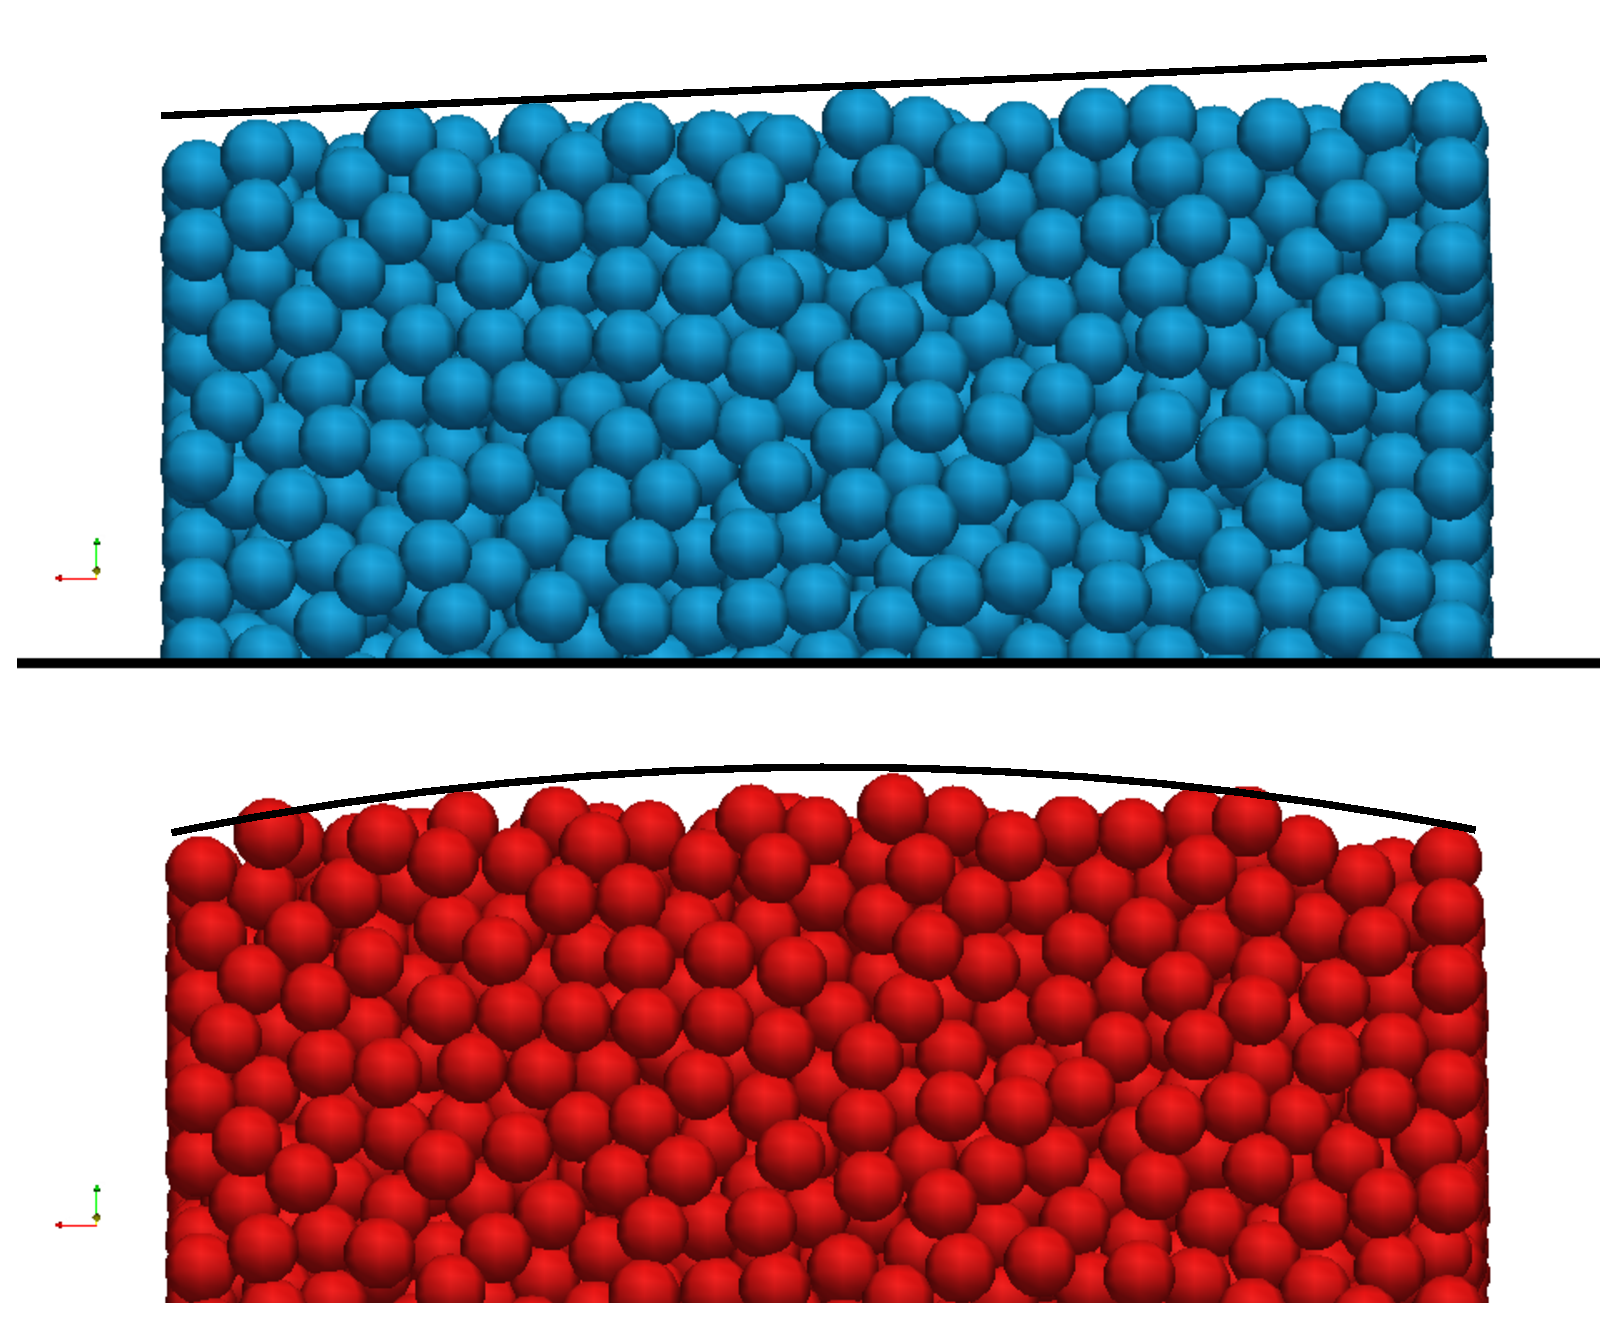
\includegraphics[width=0.5\textwidth]{chapters/figures/settlingStudy}
	\caption{Demonstrating the dynamic resettling from an example study done on location bias to pebble failure. The top image had the pebbles near the left wall biased to fail. The bottom image had a bias for the pebbles near both walls to fail. The lines are drawn as an aid to the eye.}
\label{fig:settlingStudy}
\end{figure}


The aim of this study was both to discover the impact of pebble failure on thermomechanical properties as well as determine the impact as a function of the number of failed pebbles. To satisfy the latter, we created beds with $\eta = 1\%$, $5\%$, $10\%$, and $15\%$ of pebbles failed. 

We first compare steady-state temperature profiles in the test beds against the one-dimensional theory of Eq.\ref{eq:continuum-heateqn}. To find the temperature profile in $x$, we create volumes of width $\Delta x$ that extend through the limits of the $y$- and $z$-directions. We then find the $n$ pebbles residing in the slices and take the mean value of their temperatures, $\langle T\rangle = \sum_{i}^n T_i / n$ of all pebble temperatures that have coordinates inside the slice. Below we will omit the notation $\langle T \rangle$ with the understanding that temperatures are volume-averages. Using the volume slices, we also find the average coordination number, $\langle Z \rangle = \sum_{i}^n Z_i / n$, normalized average contact force, $\langle F^* \rangle=\left[\langle F \rangle/\langle F_{bl} \rangle_\text{max}\right]^{1/3}$, and the normalized average temperature difference between pebbles in the slice, $\langle \Delta T_{ij} \rangle / (T_0 - T_s)_\text{bl}$; parameters which are discussed later.

When analytically solving Eq.~\ref{eq:thermoFirstLaw}, we introduce nondimensional temperature, $\theta_\text{1D} = (T -T_s)/(T_0-T_s)$, and spatial, $x^* = x/L$, variables and the solution becomes purely geometric; $\theta_\text{1D} = 1-x^{*2}$. We plot this theoretical solution against the temperature profiles coming from the steady-state DEM simulation in Fig.~\ref{fig:tempProfile}. We find that all our models had a nearly perfect match to a one-dimensional prediction, validating the calculation of effective thermal conductivity in this study. 

Another concern we had for pebble failure, was the phenomenon of `jamming' during resettling that would possibly leave pebbles isolated from their neighbors (apart from those they are resting upon). Such an isolated pebble would have no strong pathway for heat transfer and heat up much higher than that of its neighbors. Evidence of pebble isolation and `hot-spots' would be apparent in Fig.~\ref{fig:tempProfile} as localized deviations of data points from the quadratic profile. However, no deviations are seen in the data and we conclude that hot-spots will not be a concern in a packed bed.

\begin{figure}[htbp]
	\centering
	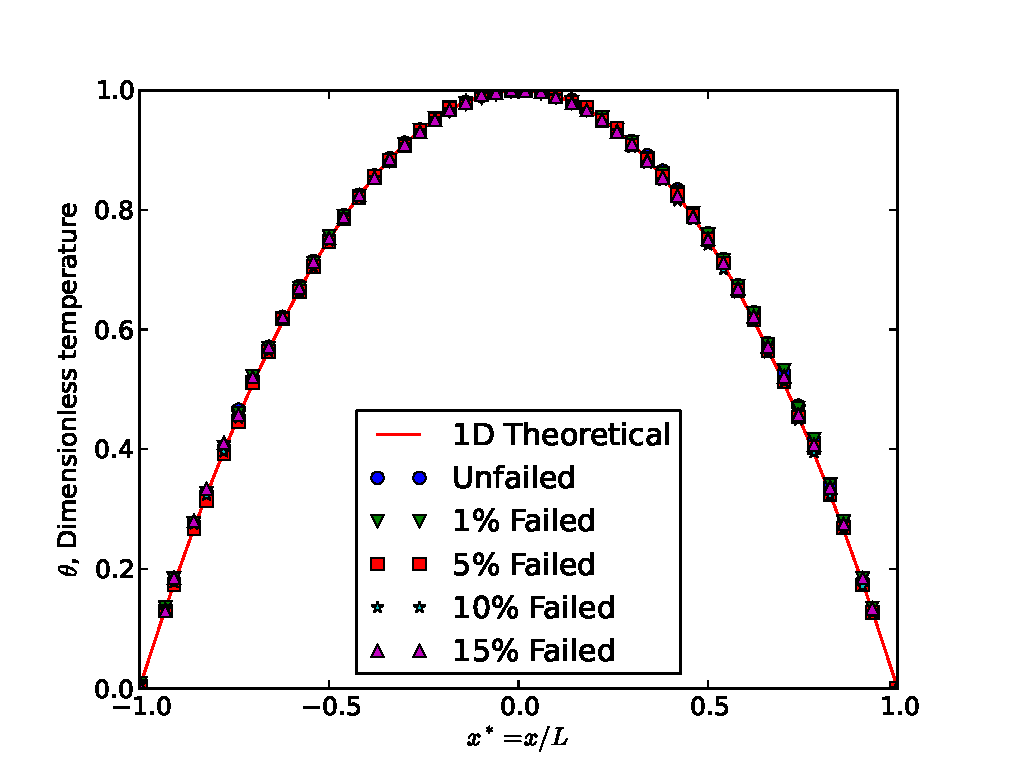
\includegraphics[width=0.65\textwidth]{chapters/figures/tempProfiles}
	\caption{The nondimensional temperature profiles for each test case follow the theoretical shape of a one-dimensional, constant $k$, continuum solution.}
\label{fig:tempProfile}
\end{figure}



\begin{figure}[htbp]
	\centering
	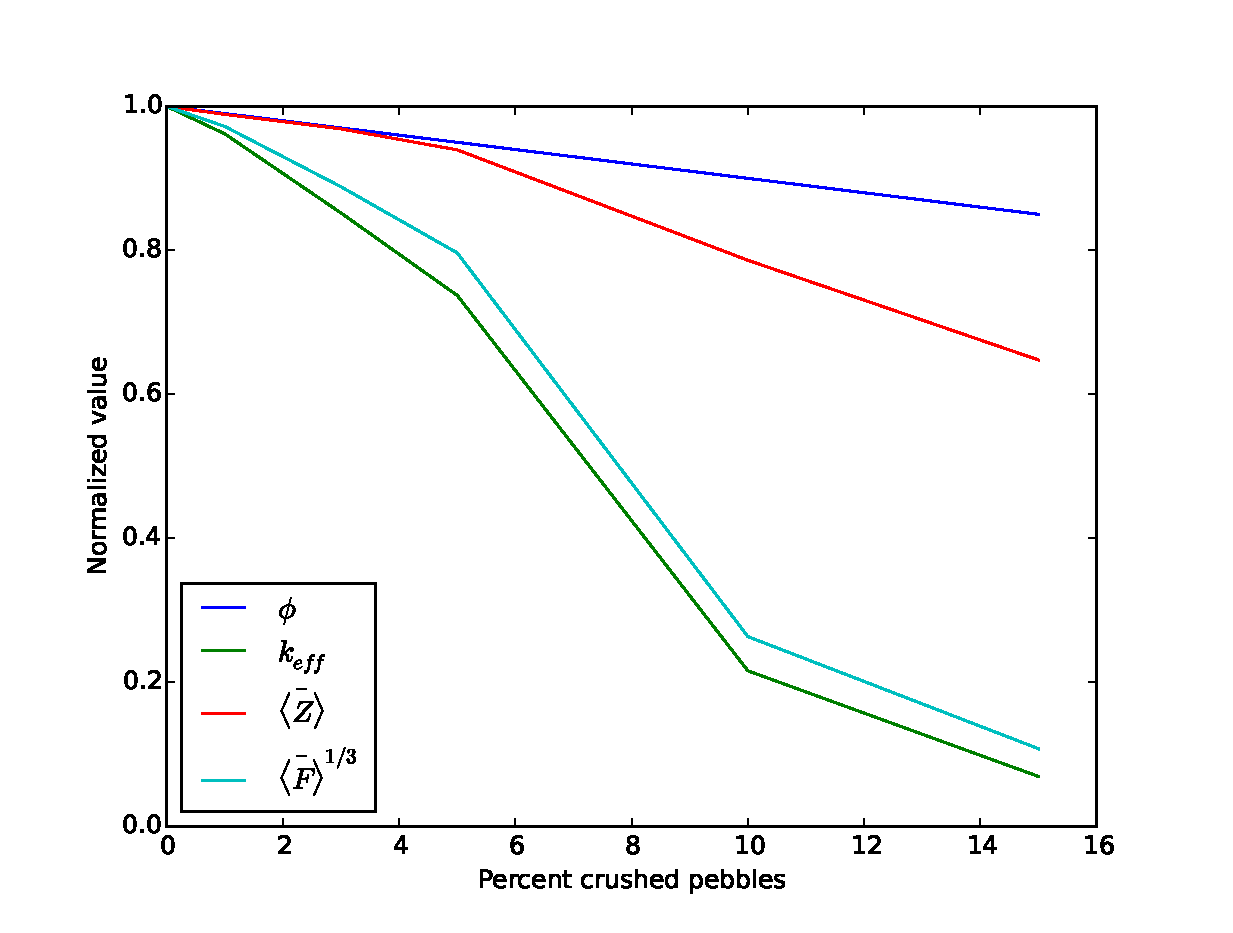
\includegraphics[width=0.65\textwidth]{chapters/figures/kEff_packingFraction}
	\caption{The normalized effective thermal conductivity (solid line) follows an exponential decay relationship with amount of failed pebbles. The normalized packing fraction (dashed line), compared to thermal conductivity, is relatively constant and is more closely fit to a linear reduction.}
\label{fig:packingFraction}
\end{figure}

\begin{figure}[htbp]
	\centering
	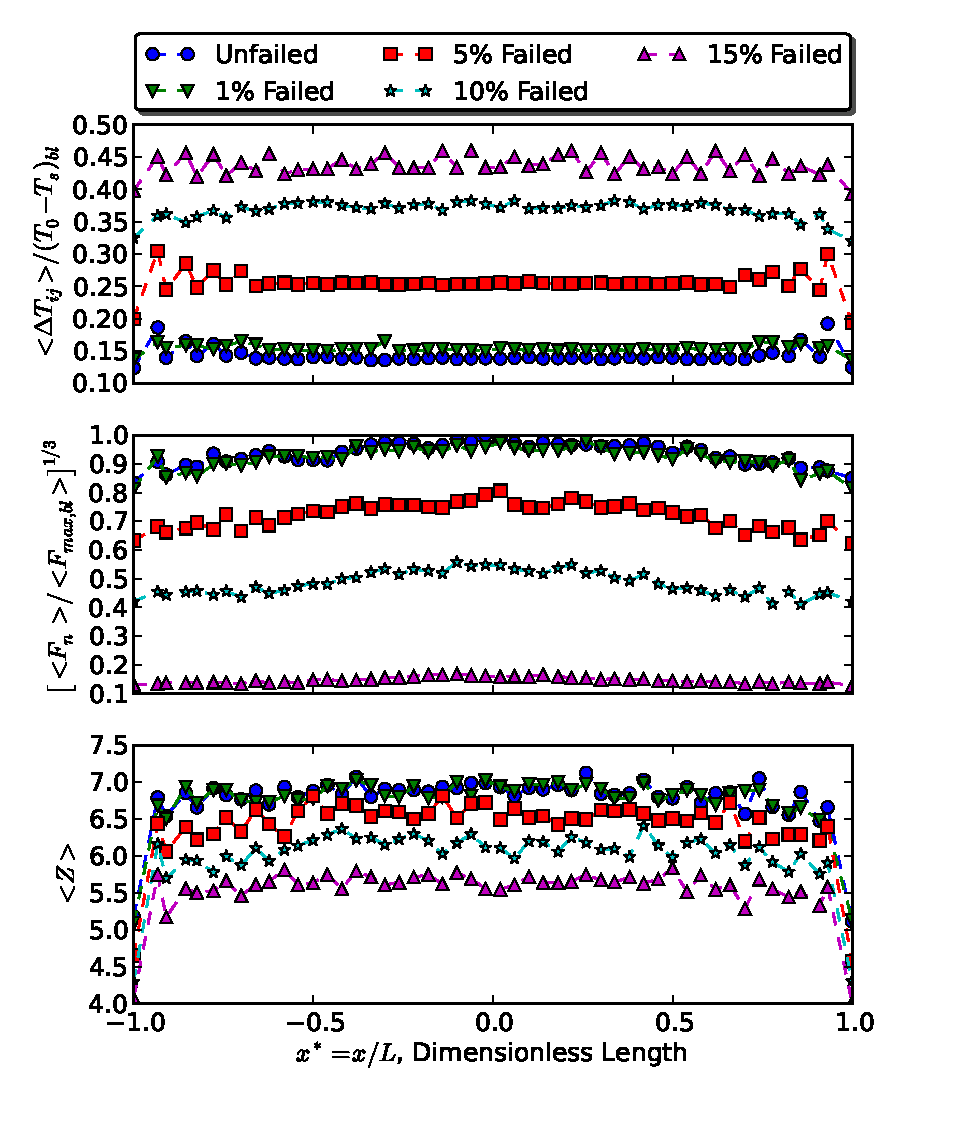
\includegraphics[width=0.75\textwidth]{chapters/figures/z_f_deltaT_subPlots}
	\caption{Average temperature differences between neighboring pebbles (top), contact forces (middle) and coordination numbers (bottom). The profiles of average coordination number and contact forces in the bed decrease in value with increasing pebble failure. Fewer and weaker contacts will reduce the possible paths of heat transfer from a pebble and this results in higher average temperatures between neighbors.}
\label{fig:coordProfiles}
\end{figure}


The effective thermal conductivity is found for all of our pebble beds, via Eq.~\ref{eq:etc}, then normalized against the conductivity of the baseline ensemble ($k_\text{eff}^* = k_\text{failed}/k_\text{bl}$). Figure~\ref{fig:packingFraction} shows the decreasing ETC with pebble failure. When $15\%$ of the pebbles are crushed in a pebble bed, the ETC has fallen all the way to only $k_\text{eff}^*=0.30$. This large reduction is especially important in light of the already poor thermal management of virgin pebble beds that, even in helium environments, have been experimentally measured at only approximately 1~W/m-K (see, { e.g.}, Refs.~\cite{Reimann:2002mi, Piazza2002}). In well-packed pebble beds, the ETC is generally related to the packing fraction. In Fig.~\ref{fig:packingFraction}, this relationship seems weak as the effective conductivity drops much more rapidly than does the packing fraction as the number of broken pebbles in the ensemble increases. To find the cause of decrease in conductivity and to make use of the information provided by DEM tools, we look to other parameters than the packing fraction.

From Eq.~\ref{eq:thermoFirstLaw}, in the steady-state, the energy input by nuclear heating must be balanced by the transport of heat out of a pebble into its neighbors. Inter-particle heat transfer is dictated by the number of neighboring contacts, temperature difference between pebbles, and the thermal conductance, $h_{ij}$ through the contact area. The thermal conductance is, itself, a function of material properties  (which are essentially constant here) and the force at the contact, going as $h_{ij} \propto F_n^{1/3}$. Thus, the net heat out is a function of the three variables as

\begin{equation}
	Q_\text{net} =f( Z, F_n^{1/3}, \Delta T)
\end{equation}



The variables affecting $Q_\text{net}$ are plotted in Fig.~\ref{fig:coordProfiles}. The average coordination number, shown in the bottom plot, decreases from a mid-line value of about 7.0 at the steady-state of the baseline case down to a mid-line value of 5.5 for the 15\% failed bed; a reduction of about 80\%. But this number doesn't compare with the large reduction in ETC which was $k_\text{eff}^*=0.30$. Clearly, there are fewer contacts in the pebble bed after failure but this alone does not account for the reduction in ETC.

Much more dramatic, seen in the center plot, is the reduction in average normal force seen by pebbles after many of the neighbors fail and are removed from the system. From the baseline down to the 15\% failed case, the contact forces are dramatically reduced to about $\langle F^* \rangle=0.1$.This reduction in force is joined by an increase in average neighbor temperatures which are 3 times higher for the bed with most failed pebbles when compared to the baseline. 

The results shown in Fig.~\ref{fig:coordProfiles} demonstrate that the heat transfer through a pebble bed is simultaneously a function of the coordination number and inter-particle contact forces -- which are both reduced as pebbles in the bed fail -- as well as the temperature difference between pebbles at steady state -- which increases as pebbles in the ensemble fail. Interestingly, when a pebble bed has lower overall inter-particle contact forces fewer particles would be expected to break. This would imply that pebble breakage is self-dampening; as pebbles begin to break the ensemble quickly relaxes and avoids future pebble failure. So while we induced failure up to $\eta = 15\%$, such large values may not occur in real beds. 

Another feature of Fig.~\ref{fig:coordProfiles} worth noting is the increase in averaged normal contact forces near the center of the bed relative to the walls. In the assumptions used to develop this simulation, we had noted the lack of localized force concentrations in a bed under an external mechanical load. However, in these results, owing to the nuclear heating temperature profile and thermal expansion of each pebble, there is a bias toward higher forces in the center of the bed. This result highlights the need for a model to predict failure initiation in place of the assumption of random pebble failure. 
%There are dramatic decreases near the walls for two reasons. The first being that contact of a pebble with a wall is not counted in the overall coordination number. The second is the forced ordering that pebbles experience near walls that is absent from the random packing in the bulk. Away from the walls, there is a clear decreasing trend in the coordination number as the pebble failure increases. From Eq.~\ref{eq:thermoFirstLaw}, the heat transfer from a pebble is a function of the number of neighbors with which the pebble is in contact. 



\subsection{Conclusions}
\label{sec:dem-conclusions}
This first study of this dissertation established the groundwork of the DEM modeling to be carried out in the other studies. We simulated a pebble bed with a specified fraction of the pebbles crushing during operation; then determining the repercussions of the missing pebbles as they affect the macroscopic property of effective thermal conductivity. We used the assumption of homogeneous, random locations of pebble failure to induce a failure routine without requiring external loads on the bed to actually induce the pebble crushing. After heating to a steady-state, an effective thermal conductivity was calculated for the pebble bed. The results show that large amounts of pebble failure correspond to large decreases in the conductive transport of energy through the pebble bed. The increase was due primarily to a drop in the inter-particle forces which lead to a large increase in temperature differences between neighboring pebbles.

As the first step in the modeling effort, there were many simplifications that had to be made in this study. We must note here the shortcomings of the assumptions and simplifications of this study before drawing any major conclusions from the results.

First, the `container walls' surrounding the pebble bed in this model are completely rigid and do not react as the swelling pebble bed presses into them while heating. The confined thermal expansion leads to very high contact forces in the pebble bed that may not be realistic. The abnormally high contact forces are most likely to be the source of the abnormally high baseline effective thermal conductivity, $k_0 = 1.03$~W/m-K. In experiments on the effective thermal conductivity of lithium ceramics in vacuum, the beds are often allowed to expand freely while heating (in at least one direction) and in vacuum were measured to be closer to $k_0 = 0.2$ W/m-K.\cite{Abou-Sena2005} Furthermore, as pointed out in the results, the initial contact force is strongly dependent on the \textit{initial packing state}. A different packing scheme was employed that resulted in the same initial packing fraction but with greatly reduced initial contact forces. 

Second, we saw from Fig.\ref{fig:temp-scatters} that the majority of the pebbles in the ensemble have their temperatures close fitting to an average curve but a number of the pebbles had less thermal contact with neighboring particles and consequently had much larger temperatures. This was true even in the baseline case of a tightly packed ($\phi = 64\%$) pebble bed. This phenomena is only possible because the contribution to heat transfer of the interstitial gas was not considered in this model. The flowing helium gas is expected to prevent any runaway temperatures of individual pebbles as it provides another route of energy transfer in the bed. This will be addressed in \cref{sec:cfd-dem-studies}.

Lastly, the pebble crushing did not conserve mass between pebble fragments and initial pebble. This is an issue we address in \cref{sec:fragmentation}, nor was there a predictive tool used to determine when pebbles would crush based on their inter-particle contact forces. We simply allowed an arbitrary number of pebbles to remove from the system. A predictive tool may not have expected even 2\% of the pebbles to be damaged, much less the 15\% we pushed the pebble bed to. The predictive tool is discussed in \cref{sec:failure-study} and will be applied to later models.

With the limitations mentioned, it is still worth discussing the results of this study in detail. The results shown in Figs.~\ref{fig:contact-forces-scatter} and~\ref{fig:coord-scatter} demonstrate that the heat transfer through a pebble bed is simultaneously a function of both the coordination number and inter-particle contact forces. The average values of both of these parameters reduced as pebbles in the bed were crushed. But by far the most important factor appears to be the inter-particle contact force. Between the baseline case and the bed with 15\% damage, the average inter-particle forces drop by an entire order of magnitude. The $\keff$ follow suit with a decrease to 10\% of the original value. Interestingly, when a pebble bed has lower overall inter-particle contact forces such as what we see when pebbles are crushed, we would predict fewer pebbles are likely to break. This result implies that pebble breakage is self-dampening; as pebbles begin to break the ensemble quickly relaxes and avoids future pebble failure. So while in this study we induced failure up to $\eta = 15\%$ without a concern for predicting if such a large amount would break, such large values may not occur in real beds during operation of a fusion reactor. 














%%%%%%%%%%%%%%%%%%%%%%%%%%%%%%%%%%%%%%%%%%%%%%%%%%%%%%%%%%%%%%%%%%%%%%%%%%%%%%%%%%%%%%%%%%%%%%
\section{Dynamically coupled CFD-DEM Study on $\keff$ of Pebble Peds with Pebble Damage}\label{sec:cfd-dem-studies}

We have established throughout this dissertation that the contribution of helium to the overall thermal transport of the ceramic pebble bed is important. Furthermore, in the DEM study on effective thermal conductivity, we discovered the appearance of many hot rattlers in the pebble bed -- even well-packed pebble beds. These pebbles heat from the volumetric source but have no outlet for the energy as their few contacts with neighbors are very light (see the scattered data of Fig.~\ref{fig:temp-scatters-zoomed}). The interstitial helium will provide another avenue for energy transport for these rattlers, potentially removing them as hot spots from the system completely. 

Therefore, in this section we work to introduce one method of coupling the discrete element method to a thermo-fluid model of helium. This first approach is to consider the helium as a continuum with volume-averaged contributions of the pebbles in each computational cell. The numerical implementation of fluid-solid interaction was outlined in \cref{sec:modeling-cfd-dem}.

\subsection{Modeling Setup, Boundary Conditions, and Coupling}
We begin with the same well-packed pebble bed set up in \cref{sec:dem-studies-effective-conductivity}. With the inclusion of helium, we only consider a single representative damaged bed, with $\eta = 10$\%. The random removal technique of inducing `damage' to the bed was again used (in the same manner as described in \cref{sec:dem-studies-effective-conductivity}). The intent is to deduce changes in thermophysical properties when helium is considered in the thermal transport network of the pebble bed -- and as a function of the morphological changes due to damaged pebbles.

The fluid domain is constructed to include an inlet and outlet region of fluid. The inlet region is 5 pebble diameters in length and the outlet is 30 pebble diameters. No-slip boundary conditions are enforced at the walls at the $x$-limits of the region. To match the DEM domain, periodic boundary conditions are used in the $y$-limits. The inlet face of the fluid is specified at a constant $\vec{v} = 0.05$~cm/s. The outlet face is specified with OpenFOAM's `inletOutlet' command with a given pressure. This boundary condition allows the inlet pressure to float to value that satisfies the specified inlet velocity and outlet pressure. The temperature is specified as a constant $T_w = 573$~K at the $x$-walls as well as the inlet condition. The outlet condition of the temperature field is similarly given to be `inletOutlet' with OpenFOAM.

The size of the CFD cells were chosen to be large enough to fit approximately 5 pebbles, for which the divided technique of computing void fraction is applicable (see \cref{sec:lag-eul-mapping}); the ratio of cell volume to particle volume was $V_\text{cell} / V_p = 7.46$. The helium, in this first model, used constant fluid properties. The values are given in Table~\ref{tab:cfd-properties}.

The Koch-Hill-Ladd drag model is employed in the style of Model B with an Archimedes pressure for buoyancy term. The terminology of these CFD coupling drag models is discussed in Ref.~\cite{Zhou2010}. The Nusselt number correlation of Li \& Mason is used for the scalar transport simulation of energy. OpenFOAM's dummy turbulence model (which is nothing more than a laminar model) is used.

An implicit time marching scheme is employed with a time step in the fluid domain of $\Delta t_f = 10^{-4}$ s. The small time step is not necessary to capture the fluid flow. The momentum equation is essentially not even transient as a steady-state laminar solution is achieved almost instantaneously in comparison to the long time span required to reach thermal steady state. The small time step is necessary for a relatively tight coupling to the pebble bed as the temperatures increase on the pebbles. Integration schemes of gradients, divergence terms, and laplacians are all Gauss linear or Gauss limitedLinear (as defined in OpenFOAM). The time step of the DEM is $\Delta t_f = 10^{-7}$ s which must be small for stability of the DEM explicit integration. The coupling between CFD and DEM domains occurs every 10 time steps of the fluid domain - equating to every 10000 in the pebble domain.

The layout of the pebble bed inside the CFD domain is shown in Figs.~\ref{fig:cfdem-domain-z}, \ref{fig:cfdem-domain-z}, and~\ref{fig:cfdem-domain-z}. Notable of the layout is how we relax the size of the meshes in the direction of the periodic boundaries. The size is permitted as there are few variations in fluid or temperature in the periodic direction. The meshes are made much smaller in the direction between cooling boundaries. In this direction ($x$-direction), we need the meshes small enough to resolve a temperature profile across the bed between centerline and cooling boundaries. We also want to capture the behavior of near-wall arrangement of the pebble bed. 

\begin {table}[htp] %
\caption{Constant fluid properties of helium purge gas in CFD-DEM coupling.}
\label {tab:cfd-properties} \centering %
\begin {tabular}{ ccccc }
\toprule %
$\nu$				&	$\alpha$				&	$k$		&	$C_p$		& $\rho$		\\
(m$^2$/s)			&	(m$^2$/s)				&	(W/m-K)	&	(J/kg-K)	& (kg/m$^3$)	\\\toprule
$4.02\times 10^{-4}$&	$6.06\times 10^{-4}$	& 	0.2		& 	5192.8		& 	0.175		\\\bottomrule
\end{tabular}
\end{table}


\begin{figure}[t]
	\centering
	\includegraphics[width=0.4\textwidth]{chapters/figures/x-side-view}
    \caption{Side view of the pebble bed as it resides in the CFD mesh. The meshes in the direction of the periodic faces are allowed to be larger than others.}\label{fig:cfdem-domain-x}
\end{figure}

\begin{figure}[t]
	\centering
	\includegraphics[width=0.4\textwidth]{chapters/figures/y-side-view}
    \caption{Front view of the pebble bed as it resides in the CFD mesh. The meshes in the direction of cooling are chosen to be large enough to fit many pebbles but small enough to provide a resolved temperature profile.}\label{fig:cfdem-domain-y}
\end{figure}

\begin{figure}[t]
	\centering
	\includegraphics[width=\singleimagewidth]{chapters/figures/z-top-view}
    \caption{Top view of the pebble bed as it resides in the CFD mesh.}\label{fig:cfdem-domain-z}
\end{figure}


While the energy transport is the main concern of the pebble bed, we perform a simple validation of the CFD-DEM routine against known pressure-drop correlations to provide confidence in the overall coupling and volume-averaging technique. After pressure drop is shown to be consistent with empirical predictions, we can go through the thermal results.
\FloatBarrier
\subsection{Pressure Drop}

Before analyzing thermal results from the CFD-DEM coupling, the system was run at various particle Reynolds numbers and the overall pressure drop of the packed bed was measured with a varied constant inlet velocity. This value was compared against the well-known Kozeny-Carman and Ergun equations; however the Kozeny-Carman is known to fit better with experimental data at very small Reynolds numbers. In Fig.~\ref{fig:cfdem-pressure-drop} we see the CFD-DEM coupling model is providing bed-scale pressure drops that match very well with Kozeny-Carman over the Reynold’s numbers applicable to helium purge flow in fusion reactors. This is the sole validation effort performed on the CFD-DEM tool.

\begin{figure}
        \centering
        \begin{subfigure}[b]{0.7\textwidth}
                \includegraphics[width=\textwidth]{chapters/figures/pressureDrops-full.png}
                \caption{Well-packed bed}
                \label{fig:pressure-drop-full}
        \end{subfigure}%
        
          %add desired spacing between images, e. g. ~, \quad, \qquad, \hfill etc.
          %(or a blank line to force the subfigure onto a new line)
        \begin{subfigure}[b]{0.7\textwidth}
                \includegraphics[width=\textwidth]{chapters/figures/pressureDrops-evap.png}
                \caption{Re-settled bed}
                \label{fig:pressure-drop-evap}
        \end{subfigure}
        \caption{Pressure drop calculations across packed beds, solved by CFD-DEM, fit well to the Kozeny-Carman empirical relation.}\label{fig:cfdem-pressure-drop}
\end{figure}
\subsection{Effective Thermal Conductivity from CFD-DEM}\label{sec:cfd-dem-effective-conductivity}

The simulation is allowed to run to thermal steady-state with nuclear heating and wall cooling. After reaching a steady solution, I analyze the temperature profiles of the fluid and pebble bed. The temperature of the fluid volume from the simulation of the well-packed bed is shown in Fig.~\ref{fig:cfdem-complete-domain}. The flow field is also visualized in Fig.~\ref{fig:cfdem-streamlines}; in this figure the pebble bed is clipped at the centerline to allow viewing of the helium streamlines. Apparent in the figure is temperature profiles in the helium from centerline to wall that qualitatively mirror temperature profiles in the pebble bed. The two beds in our system, well-packed and resettled, were run to thermal steady-state with nuclear heating and wall cooling in both pure DEM and coupled CFD-DEM simulations for comparison. From steady-state temperature distributions, seen in the pebble scatter plots in Fig.~\ref{fig:cfdem-x-T}, an average profile is calculated and an effective thermal conductivity computed following the procedure shown in \cref{sec:keff-analogy}. The values are tabulated in Table~\ref{tab:cfdem-keff}. 

In the case of pure DEM, energy is transported solely along conduction routes in the ensemble. When the packing of the bed is disturbed, this results in a substantial drop in effective conductivity (a drop of 31\%). Perhaps more important than the reduction in effective conductivity, is the growth in number of isolated rattlers. Because heat deposition is volumetrically applied, pebbles with poor conduction routes become much hotter than their neighbors. This is evident in the high temperatures seen in many of the pebbles in the Fig.~\ref{fig:x-T-evap}. Over-heating of isolated pebbles could induce sintering and impact their tritium release even when the average temperatures measured in the bed are well below sintering values.

When CFD-DEM beds are analyzed, there is still a large reduction in effective conductivity (22\% drop), but interesting to note is the lack of high temperature rattlers. In the CFD-DEM scatter plot of Fig.~\ref{fig:x-T-evap}, there is evidence of the reduced heat transfer in the same region as the isolated pebbles from the DEM bed, but the temperatures are much closer to the average values of neighboring pebbles. The helium purge gas has locally smoothed out the temperatures and provided heat transport paths for pebbles that have loose physical contact with neighbors.

In spite of the 22\% decrease in effective conductivity, the maximum temperature of the pebble bed only increased 6.2\% (from \SIlist{725;751}{\kelvin} when helium is included in the model. This result is significant for solid breeder designers. They may choose a solid breeder volume such that in the event of extensive pebble cracking, the maximum temperature of the bed would remain within the ideal windows dictate for the lithium ceramics.

An accompanying result is the increased amount of energy carried out of the system by the helium purge gas. In Table I, the last column provides the ratio of energy carried out of the system to the nuclear energy deposited into the bed. The amount of energy carried out by the helium increased from \numlist{1.15;1.52}\% from the well-packed to damaged beds.

\begin{figure}[t]
    \centering
    \includegraphics[width=\singleimagewidth]{chapters/figures/full-cfd-dem-fluid-temp}
    \caption{View of the complete fluid domain at thermal steady state.}\label{fig:cfdem-complete-domain}
\end{figure}


\begin{figure}[t]
    \centering
    \includegraphics[width=\singleimagewidth]{chapters/figures/cfd-dem-streamlines2}
    \caption{Cut-away view of the pebble bed with streamlines of helium moving in generally straight paths from inlet to exit.}\label{fig:cfdem-streamlines}
\end{figure}


\begin{figure}
        \centering
        \begin{subfigure}[b]{0.5\textwidth}
                \includegraphics[width=\textwidth]{chapters/figures/full-x-T-color}
                \caption{Well-packed bed}
                \label{fig:x-T-full}
        \end{subfigure}%
        
          %add desired spacing between images, e. g. ~, \quad, \qquad, \hfill etc.
          %(or a blank line to force the subfigure onto a new line)
        \begin{subfigure}[b]{0.5\textwidth}
                \includegraphics[width=\textwidth]{chapters/figures/evap-x-T-color}
                \caption{Re-settled bed}
                \label{fig:x-T-evap}
        \end{subfigure}
        \caption{Scatter temperature profiles of pebbles in a bed that is: well-packed (left) and resettled after 10\% of pebbles were removed from crushing (right). The introduction of helium into the simulation contributes to both lower overall temperatures (higher effective conductivity) and the smoothing out of high temperatures of isolated pebbles.}\label{fig:cfdem-x-T}
\end{figure}



\begin {table}[htp] %
\caption{Pebble bed values from the test matrix of the beds analyzed in this study.}
\label {tab:cfdem-keff} \centering %
\begin {tabular}{ rccccc }
\toprule %
			& 	\multicolumn{2}{c}{$\keff$}	&   \multicolumn{2}{c}{$T_\text{max}$}	&	$\frac{Q_h}{Q_\text{nuc}}$		\\
			& 	\multicolumn{2}{c}{(\si{\watt\per\meter\per\kelvin})}			&	\multicolumn{2}{c}{(\si{\kelvin})}				&									\\
			& 	DEM 		& 	CFD-DEM				&	DEM 		& 	CFD-DEM 			& 	CFD-DEM							\\\toprule
Well-packed	& 	0.96		& 	1.09				& 	745			& 	725					& 	1.15							\\
Resettled	& 	0.66		& 	0.85				& 	800			& 	751					& 	1.52							\\\bottomrule
\end{tabular}
\end{table}





\FloatBarrier



\subsection{Conclusions}
The CFD-DEM formulation maintains calculations of pebble-pebble interactions while dynamically coupling to the helium flow. The model demonstrates the ability of helium gas to smooth out any hot spots predicted by pure-conduction DEM formulations. Further, the lattice-Boltzmann simulation, while not fully coupled to DEM, revealed important features of helium flow in volumetrically heated pebble beds – mainly the smearing of temperature profiles along the paths of cooling.










%%%%%%%%%%%%%%%%%%%%%%%%%%%%%%%%%%%%%%%%%%%%%%%%%%%%%%%%%%%%%%%%%%%%%%%%%%%%%%%%%%%%%%%%%%%%%%
\section{3D Lattice-Boltzmann Models of the Complete Conjugate Heat Transfer of Helium Purge Gas and Ceramic Pebble Beds}\label{sec:lbm-studies}

%\input{chapters/sections/lbm-studies-effective-conductivity.tex}

\section{Discussion \& Conclusions}
Single largest factor determining effective conductivity (in a pure conduction environment) is contact force
In simple model of removed particles, a non-linear reduction in effective conductivity was observed
Size and complexity of porous bed make it impractical for modeling conjugate heat transfer on pebble-scale with conventional CFD tools
Introduced two efficient methods for modeling helium purge gas interacting with packed beds
Directly coupled CFD-DEM for volume-averaged fluid-pebble and discrete pebble-pebble interactions
DEM packing structures imported into LBM simulations for more detailed modeling of fluid flow and thermal transport
Significant results from models of our test cases:
Discovered laminar mixing in packed beds with volumetric heating and wall cooling broadens/flattens temperature profiles in the bed 
‘Rattlers’ have their temperatures regulated by helium
Laminar mixing of energy has many promising features not expected from the helium purge gas in breeder blankets